\section* {2.1  Методы простой итерации и Ньютона}

\subsection{Постановка задачи}
Реализовать методы простой итерации и Ньютона решения нелинейных уравнений в виде программ, задавая в качестве входных данных точность вычислений. С использованием разработанного программного обеспечения найти положительный корень нелинейного уравнения (начальное приближение определить графически). Проанализировать зависимость погрешности вычислений от количества итераций.

{\bfseries Вариант:} 26

$lg(x+1)-x+0.5=0$
%\pagebreak

\subsection{Результаты работы}
\begin{figure}[h!]
\centering
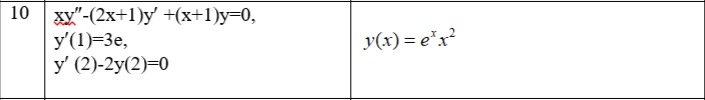
\includegraphics[width=12cm, height=6cm]{img1}
\caption{Вывод программы в консоли}
\end{figure}
\pagebreak

\subsection{Исходный код}

\lstinputlisting{include/lab2-1.c}
\pagebreak

\section* {2.2  Методы простой итерации и Ньютона}

\subsection{Постановка задачи}
Реализовать методы простой итерации и Ньютона решения систем нелинейных уравнений в виде программного кода, задавая в качестве входных данных точность вычислений. С использованием разработанного программного обеспечения решить систему нелинейных уравнений (при наличии нескольких решений найти то из них, в котором значения неизвестных являются положительными); начальное приближение определить графически. Проанализировать зависимость погрешности вычислений от количества итераций. 

{\bfseries Вариант:} 26

\begin{cases}
& 2x_1^2-x_2+x_2^2-2 = 0 \\
& x_1-\sqrt{x_2+2}+1 = 0 \\
\end{cases}
%\pagebreak

\subsection{Результаты работы}
\begin{figure}[h!]
\centering
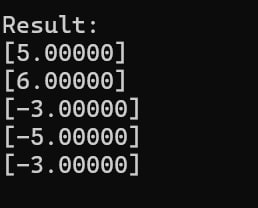
\includegraphics[width=15cm, height=6cm]{img2}
\caption{Вывод программы в консоли}
\end{figure}
\pagebreak


\subsection{Исходный код}

\lstinputlisting{include/lab2.h}
\lstinputlisting{include/lab2.c}
\lstinputlisting{include/lab2-2.c}
